\documentclass[aspectratio=169]{beamer}
\input{imsb_beamer.tex}
\usepackage{graphicx}
\graphicspath{{figs/}}

\title{Spatial transcriptomics of kidney: a Xenium glomerulonephritis workflow}
\author{Robin Khatri}
\institute{Institute of Medical Systems Bioinformatics, UKE}
\date{June 2026}

\begin{document}

\begin{frame}[plain]\titlepage\end{frame}

\begin{frame}{Format}
  One day face to face; the notebooks are an end-to-end reference you keep working through.
  \vskip0.4em
  \begin{itemize}
    \item We analyse one real Xenium kidney slide: 480-gene panel, FFPE, 8 tissue samples
      from three glomerulonephritis (GN) types.
    \item Six notebooks: read and split the slide, transcriptomics, classification,
      integration, differential expression, spatial analysis.
    \item Each notebook carries method notes and interpretation; solutions are revealed later.
  \end{itemize}
\end{frame}

\begin{frame}{Why spatial, and why these samples}
  \begin{columns}[T]
  \begin{column}{0.56\textwidth}
  Dissociated scRNA-seq tells you \emph{which} cells are present; the kidney's function and
  its diseases live in \emph{where} they are: glomeruli, tubules, and immune foci.
  \vskip0.4em
  The slide carries 8 cores from three immune-mediated GN types:
  \begin{itemize}
    \item \textbf{ANCA-GN} (necrotising/crescentic), 5 samples
    \item \textbf{anti-GBM} (GBM), 1 sample
    \item \textbf{Lupus nephritis} (SLE), 2 samples
  \end{itemize}
  No healthy control is on this slide, so we contrast \emph{ANCA-GN vs the other GN types}.
  \end{column}
  \begin{column}{0.42\textwidth}
  \small
  \textbf{Xenium in one line.} An imaging assay that localises individual transcripts of a
  targeted panel and assigns them to cells by segmentation: single-cell resolution, limited
  gene set, with coordinates kept.
  \end{column}
  \end{columns}
\end{frame}

\begin{frame}{One slide, eight samples}
  \begin{columns}[T]
  \begin{column}{0.48\textwidth}
  \centering
  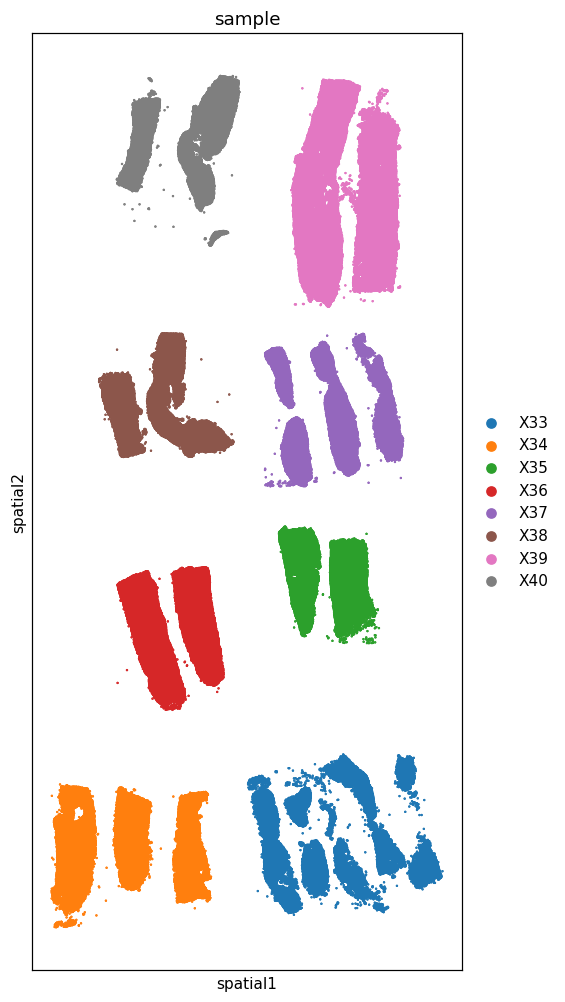
\includegraphics[height=0.78\textheight]{fig_samples.png}
  \end{column}
  \begin{column}{0.5\textwidth}
  \small
  The 8 samples are separate tissue cores in one shared coordinate system. We split them with
  per-sample \textbf{bounding boxes} (`data/sample\_bounding\_boxes.csv`), derived from an
  independent, careful segmentation of the same slide: the cell barcodes differ, but the
  micron coordinates match, so the boxes transfer to the raw data.
  \vskip0.3em
  Each raw cell is assigned to the box that contains its centroid; the few cells in the gaps
  between cores are dropped.
  \end{column}
  \end{columns}
\end{frame}

\begin{frame}{Quality control}
  \centering
  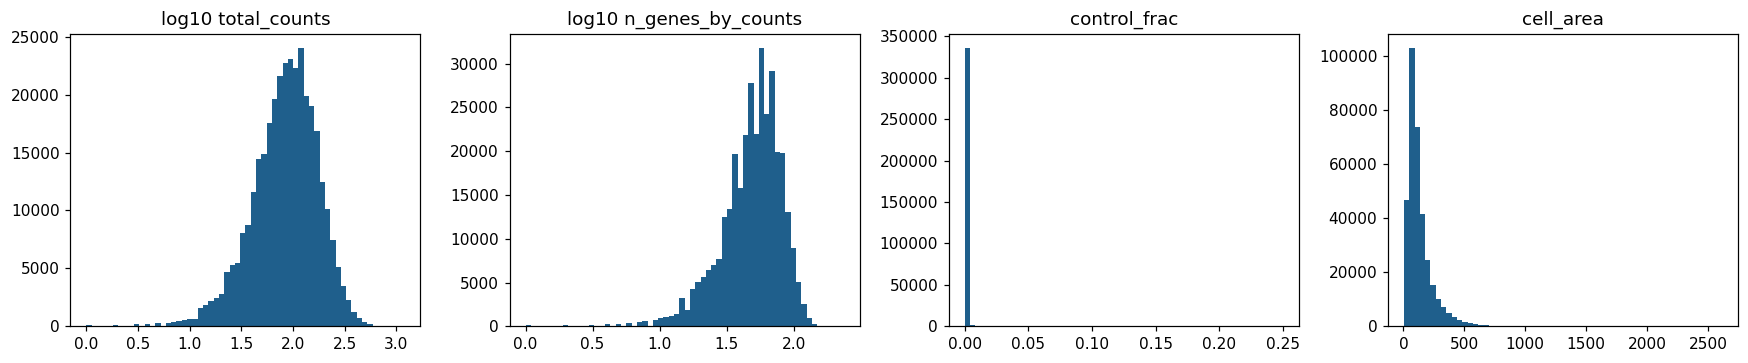
\includegraphics[width=0.95\linewidth]{fig_qc.png}
  \vskip0.3em
  \footnotesize
  Transcripts and genes per cell (coverage / fragmented segments), control fraction (noise
  floor), and cell area (segmentation). Read the distributions and the per-sample summary
  before choosing thresholds; watch for a sample that stands apart for technical reasons.
\end{frame}

\begin{frame}{Annotation 1: clustering and markers}
  \begin{columns}[T]
  \begin{column}{0.5\textwidth}
  \centering
  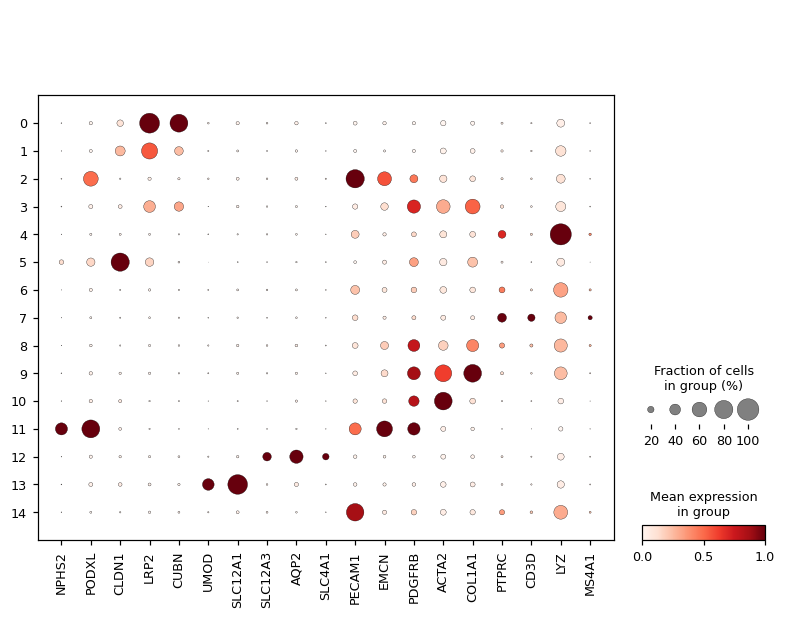
\includegraphics[width=\linewidth]{fig_markers_dotplot.png}
  \end{column}
  \begin{column}{0.48\textwidth}
  \small
  Cluster (Leiden) on the 480-gene panel (too few genes to select HVGs), then name clusters
  from \textbf{marker scores}: each cluster takes the lineage whose markers it expresses most.
  Transparent and reference-free, but coarse, the panel bounds what you can resolve.
  \vskip0.3em
  Check the dotplot: do clusters light up the canonical kidney markers (NPHS2/PODXL for
  podocytes, LRP2/CUBN for proximal tubule, UMOD for TAL, PECAM1 for endothelium)?
  \end{column}
  \end{columns}
\end{frame}

\begin{frame}{Cell types in space}
  \begin{columns}[T]
  \begin{column}{0.5\textwidth}
  \centering
  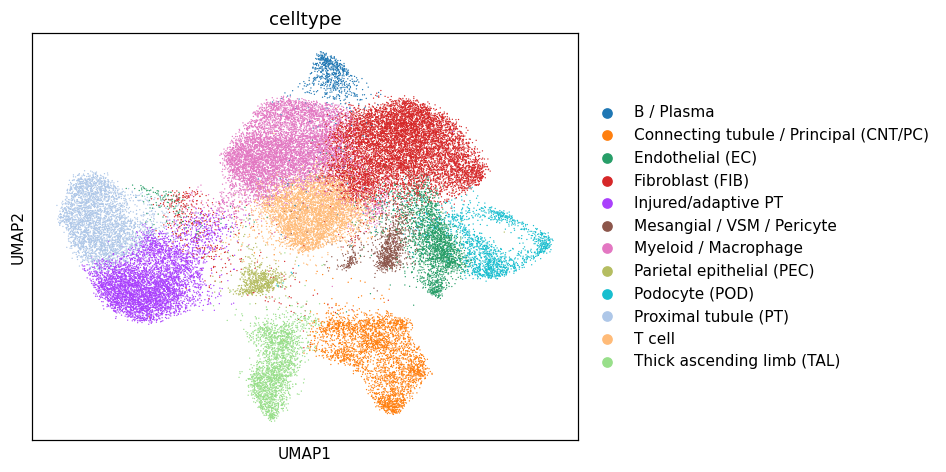
\includegraphics[width=\linewidth]{fig_celltype_space.png}
  \end{column}
  \begin{column}{0.5\textwidth}
  \centering
  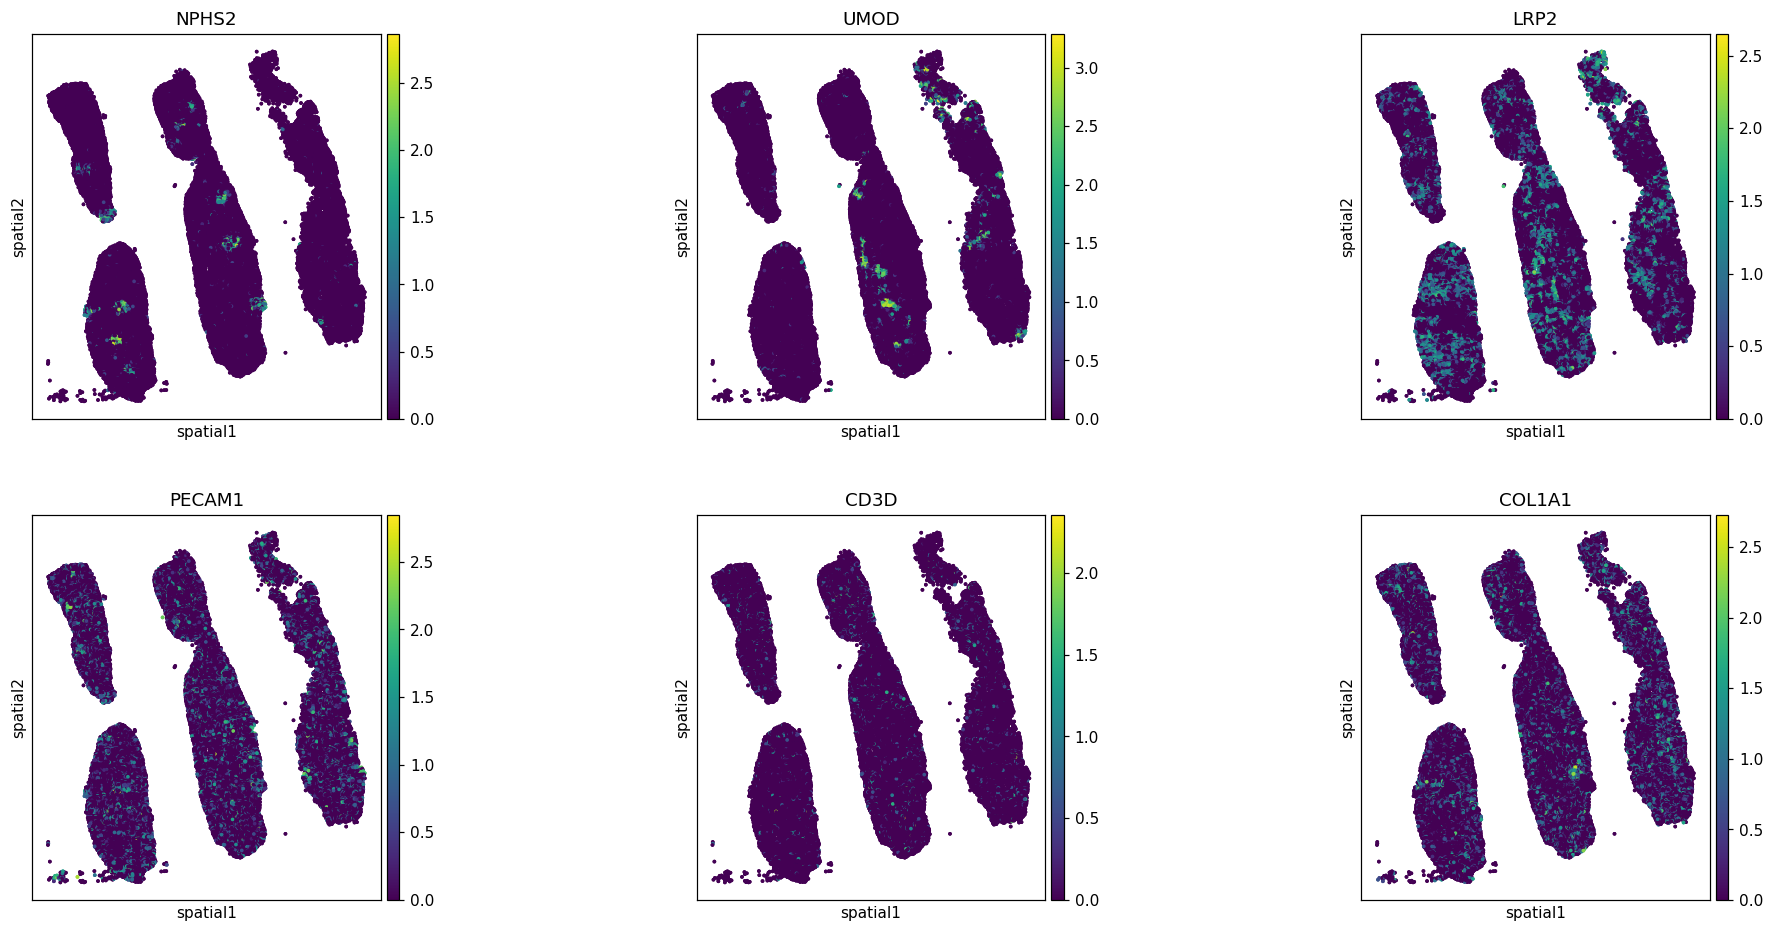
\includegraphics[width=\linewidth]{fig_marker_genes_space.png}
  \end{column}
  \end{columns}
  \vskip0.2em
  \footnotesize
  The UMAP groups cells transcriptionally; the tissue plot checks they form sensible
  structures. Tubule types should trace tubules, podocytes sit in glomerular tufts, immune
  cells are interstitial. A label that scatters where it should be structured is suspect.
\end{frame}

\begin{frame}{Annotation 2: markers vs a reference}
  \begin{columns}[T]
  \begin{column}{0.5\textwidth}
  \centering
  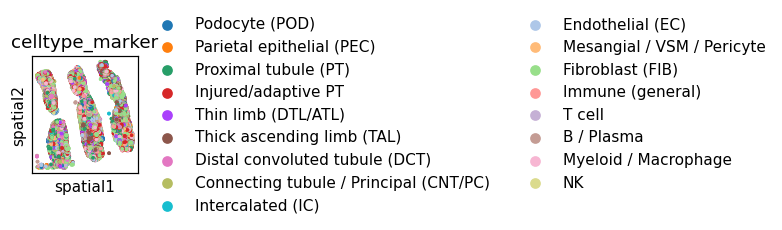
\includegraphics[width=\linewidth]{fig_class_marker.png}\\
  {\scriptsize marker-based (reference-free)}
  \end{column}
  \begin{column}{0.5\textwidth}
  \centering
  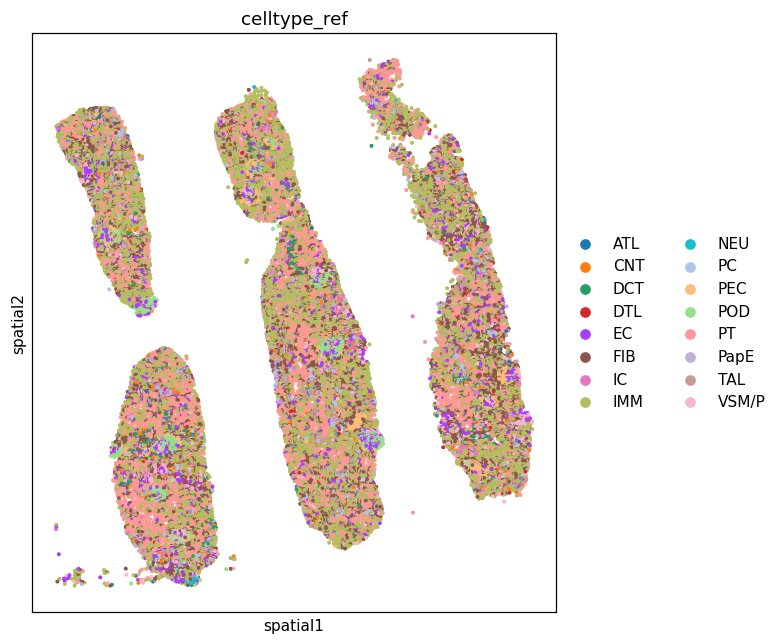
\includegraphics[width=\linewidth]{fig_class_ref.png}\\
  {\scriptsize reference-based (Lake/KPMP classifier)}
  \end{column}
  \end{columns}
  \vskip0.2em
  \footnotesize
  A logistic-regression classifier trained on the Lake/KPMP snRNA-seq atlas (`subclass.l1`,
  shared panel genes) transfers finer labels with a confidence. \textbf{Caveat}: a snRNA-seq vs
  imaging platform gap, and it ignores spatial context, hence integration next.
\end{frame}

\begin{frame}{Integration: align samples before comparing}
  \begin{columns}[T]
  \begin{column}{0.56\textwidth}
  \centering
  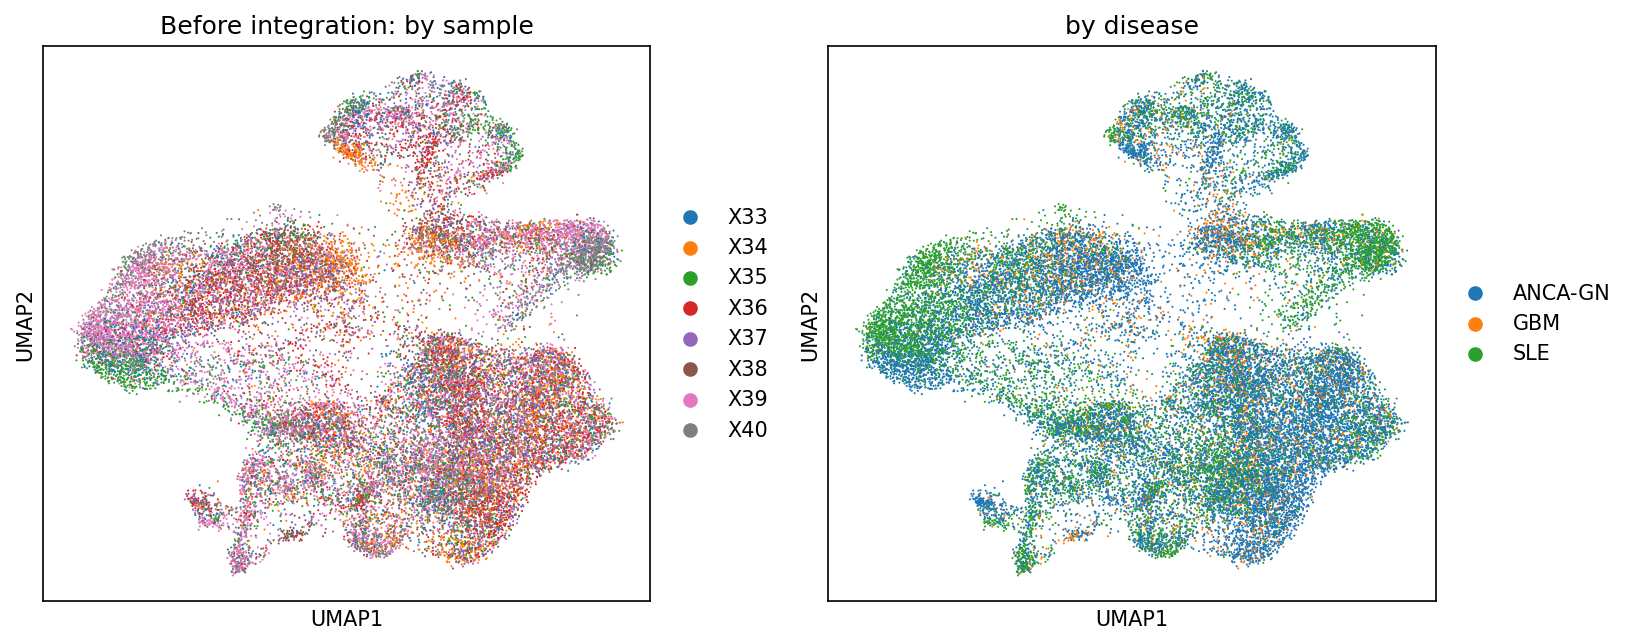
\includegraphics[width=\linewidth]{fig_int_pre.png}
  \end{column}
  \begin{column}{0.42\textwidth}
  \small
  Before correction, cells separate partly by \textbf{sample/disease}: a batch effect mixed
  with real biology. \textbf{Harmony} (CPU) aligns the embeddings so the same cell type
  overlaps across samples; scVI/scANVI are GPU alternatives. The risk is \textbf{over-correction}
  erasing real differences, so check that cell types and markers stay put.
  \end{column}
  \end{columns}
\end{frame}

\begin{frame}{Composition by disease}
  \centering
  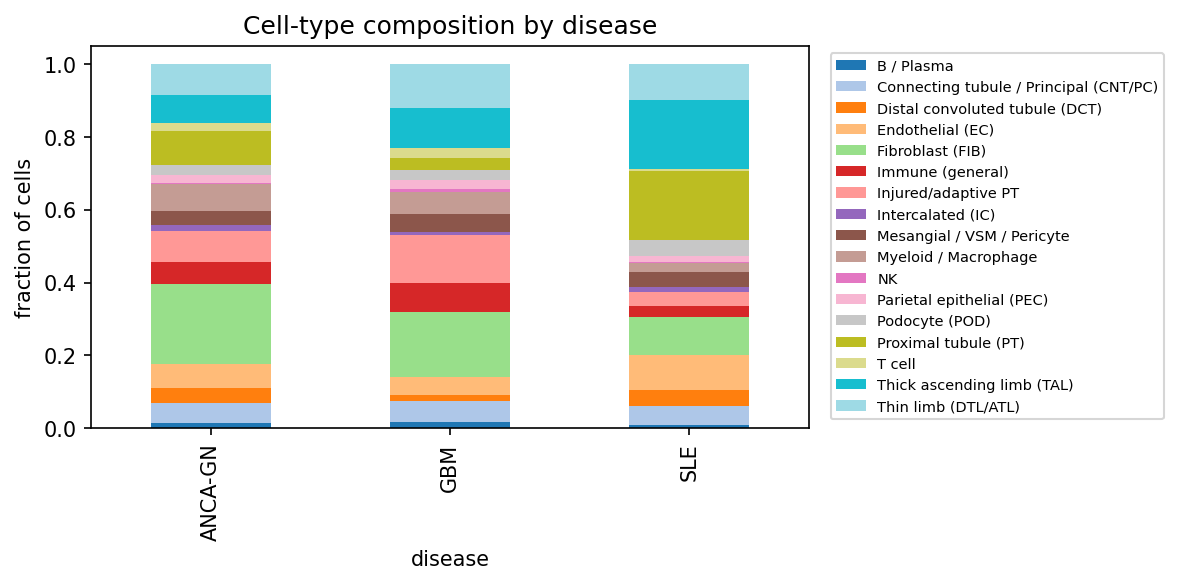
\includegraphics[width=0.8\linewidth]{fig_composition.png}
  \vskip0.2em
  \footnotesize
  With cells aligned, compare cell-type fractions across groups. Read it as descriptive:
  proportions move with tissue sampling and the groups are small (5 ANCA-GN, 1 GBM, 2 SLE).
  The next step tests differences with the sample as the unit of replication.
\end{frame}

\begin{frame}{Differential expression: ANCA-GN vs other GN}
  \begin{columns}[T]
  \begin{column}{0.52\textwidth}
  \centering
  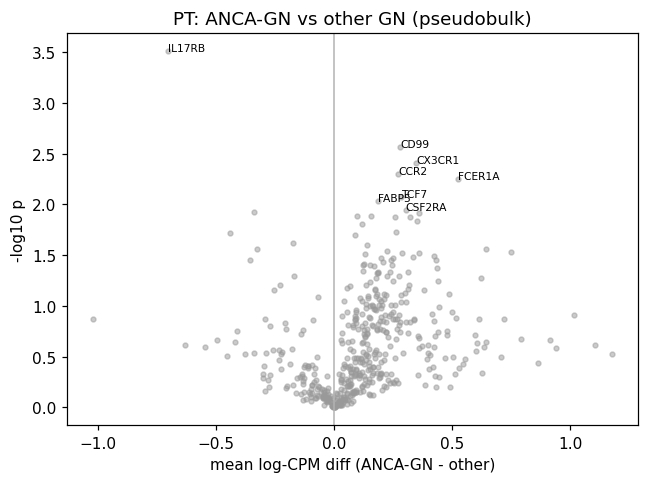
\includegraphics[width=\linewidth]{fig_volcano.png}
  \end{column}
  \begin{column}{0.46\textwidth}
  \small
  \textbf{Pseudobulk}: sum counts per sample $\times$ cell type and test across \emph{samples}.
  Per-cell DE would treat tens of thousands of cells from a few biopsies as independent
  (pseudoreplication) and vastly overstate significance.
  \vskip0.3em
  With 5 vs 3 samples and no healthy control, treat hits as exploratory; a curated
  over-representation test then reads which programmes (inflammation, complement, fibrosis,
  endothelial activation) the changes touch.
  \end{column}
  \end{columns}
\end{frame}

\begin{frame}{Spatial: neighbourhood enrichment}
  \begin{columns}[T]
  \begin{column}{0.52\textwidth}
  \centering
  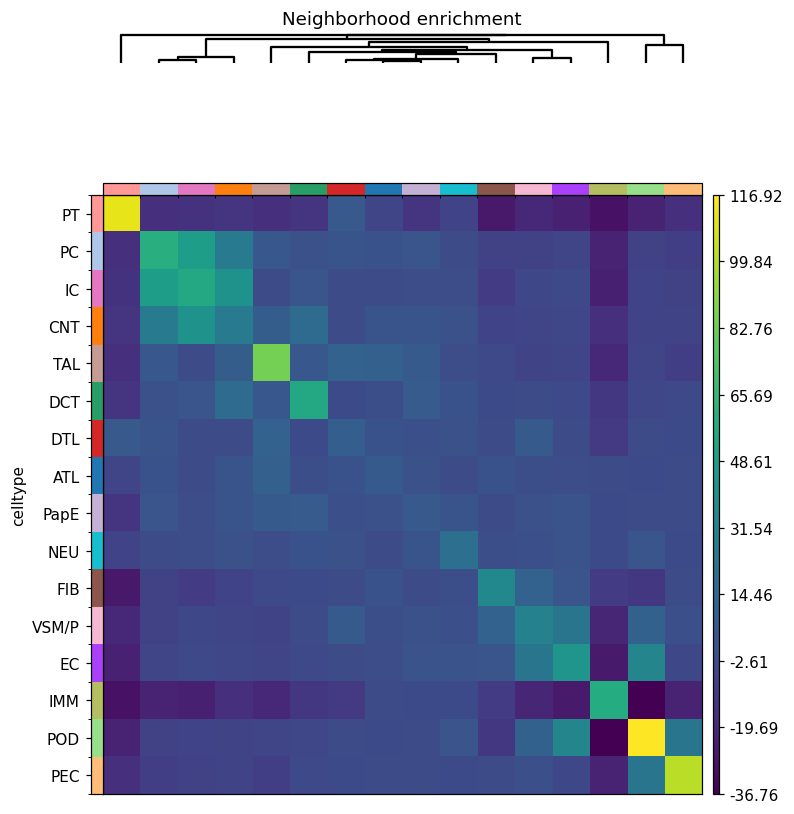
\includegraphics[width=\linewidth]{fig_nhood.png}
  \end{column}
  \begin{column}{0.46\textwidth}
  \small
  Permute cell-type labels on the spatial graph and compare adjacency to the null (z-score).
  The diagonal is self-aggregation; positive off-diagonal pairs co-locate (immune cells around
  injured tubules or vessels), negative pairs avoid each other.
  \vskip0.3em
  It is relative to this core's composition and the chosen graph, so compare like with like
  across samples.
  \end{column}
  \end{columns}
\end{frame}

\begin{frame}{Spatial: niches}
  A niche is a recurring local cell-type mixture. \textbf{Composition-based} clusters each cell's
  neighbourhood mix; \textbf{BANKSY-style} augments expression with the neighbour mean. They should
  agree on the major compartments (glomeruli, tubulo-interstitium, immune foci).
  \vskip0.2em
  \begin{columns}[T]
  \begin{column}{0.5\textwidth}
  \centering
  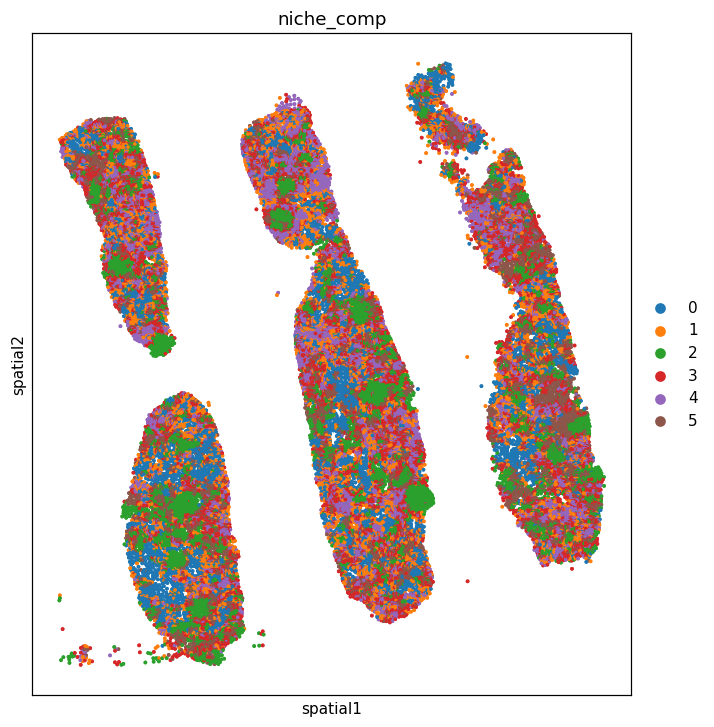
\includegraphics[width=0.74\linewidth]{fig_niche_comp.png}\\
  {\scriptsize composition-based}
  \end{column}
  \begin{column}{0.5\textwidth}
  \centering
  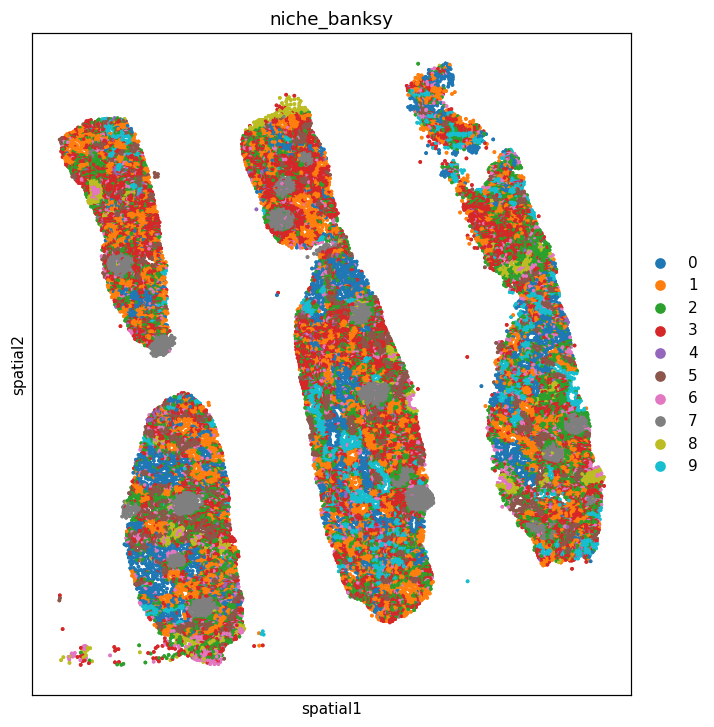
\includegraphics[width=0.74\linewidth]{fig_niche_banksy.png}\\
  {\scriptsize BANKSY-style}
  \end{column}
  \end{columns}
\end{frame}

\begin{frame}{Spatial: ligand-receptor interactions}
  \centering
  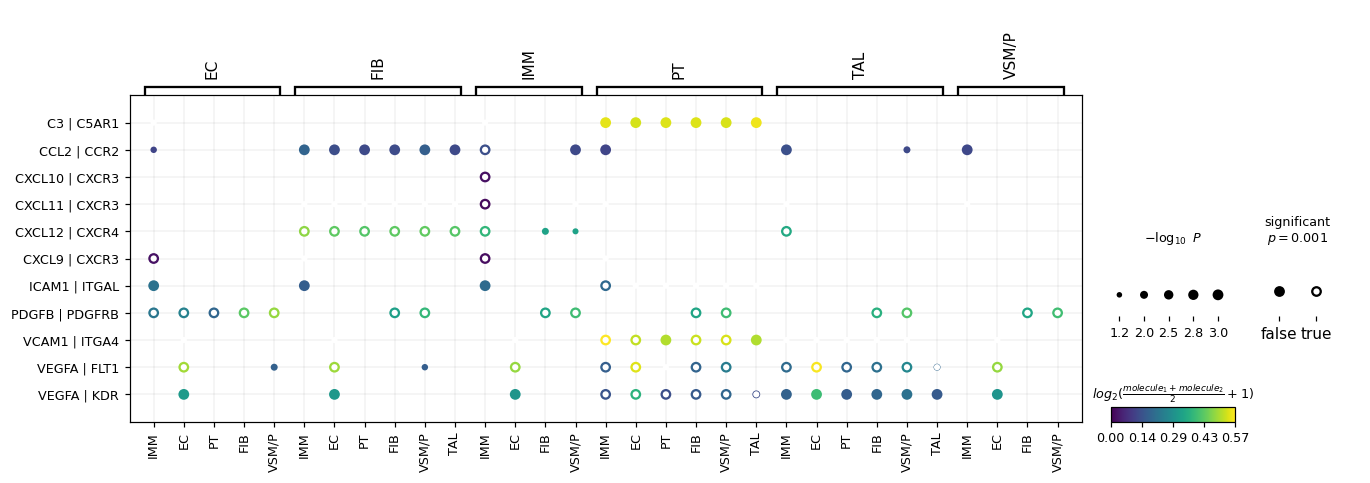
\includegraphics[width=0.96\linewidth]{fig_ligrec.png}
  \vskip0.2em
  \footnotesize
  For each sender $\to$ receiver cell-type pair, test whether a ligand and its receptor are
  co-expressed more than chance (permutation). On a targeted panel only curated pairs are
  measurable (e.g.\ CXCL9/10/11 $\to$ CXCR3 recruiting T cells). Expression is a proxy for
  activity, and segmentation error can move a ligand to the wrong cell, so read hits as
  hypotheses.
\end{frame}

\begin{frame}{Reading results critically}
  \begin{itemize}
    \item \textbf{Replication is the sample, not the cell.} Per-cell tests overstate significance;
      use pseudobulk and composition-aware methods.
    \item \textbf{Small n, no control.} Five ANCA-GN vs three other-GN samples, no healthy tissue:
      contrasts are between GN types and are exploratory.
    \item \textbf{Segmentation and panel.} Misassigned transcripts corrupt typing and
      communication; absent genes are weak evidence.
    \item \textbf{Everything spatial is conditional} on the graph and the section. Compare across
      samples before drawing disease conclusions.
  \end{itemize}
\end{frame}

\begin{frame}{The workflow, and where to go next}
  \centering
  \begin{tikzpicture}[node distance=4mm,every node/.style={box,minimum height=0.8cm,text width=1.9cm,font=\scriptsize}]
    \node (a) {split + QC};
    \node[right=of a] (b) {cluster + markers};
    \node[right=of b] (c) {reference classify};
    \node[right=of c] (d) {integrate};
    \node[below=7mm of d] (e) {DE + enrichment};
    \node[left=of e] (f) {spatial / niches};
    \node[left=of f] (g) {interpret};
    \draw[arr] (a)--(b); \draw[arr] (b)--(c); \draw[arr] (c)--(d);
    \draw[arr] (d)--(e); \draw[arr] (e)--(f); \draw[arr] (f)--(g);
  \end{tikzpicture}
  \vskip0.5em
  \footnotesize
  The six notebooks follow this path on the real slide. Beyond the course: scANVI/scVI
  integration, whole-transcriptome enrichment (decoupler/gseapy + MSigDB), dedicated niche tools
  (BANKSY, CellCharter), and a healthy-control cohort for true case-control contrasts.
\end{frame}

\end{document}
